\label{cap:normativa}

En este capítulo, se pretende identificar la normativa estatal, autonómica y local que regula las características de las vías accesibles, así como extraer los parámetros que se necesitan recopilar y medir en la práctica. Se considera únicamente la normativa aplicable a las calles, dejando fuera la normativa de los edificios.
\\

Una vez analizado el marco legal, se describirán los diferentes conceptos, medidas específicas y elementos que conforman una calle accesible, y se identificarán aquellas características que pueden ser potencialmente extraídas de las imágenes aéreas o a pie de calle, y cuáles son únicamente observables mediante inspección in situ.
\\

\section{Marco legal y normativo}

\label{sec:marco-legal}
Se procede a analizar y describir el marco legal desde la normativa más general a la más específica, comenzando por el ámbito internacional, siguiendo con el estatal y posteriormente el autonómico (Andalucía y Castilla-La Mancha) y local (Algeciras y Albacete).

\subsection{Marco internacional}
La \textbf{Convención Internacional sobre los derechos de las personas con discapacidad} (Naciones Unidas, 2006) constituye un punto de inflexión en la accesibilidad, puesto que estableció de manera internacional los derechos de las personas con discapacidad, pasando de un enfoque asistencial a considerarlas personas de plenos derechos. Además, subraya la necesidad de incorporar una perspectiva de género en todas las políticas y destaca la discriminación adicional que sufren las mujeres (artículo 6).
\\

Se establecen los derechos fundamentales de las personas con discapacidad, incluyendo plena igualdad de oportunidades, accesibilidad, participación plena y efectiva, y no discriminación.
\\

Concretamente, el artículo 9 de la Convención obliga formalmente a los estados a transformar el entorno físico, el transporte, la información o las comunicaciones para que sean accesibles para todas las personas.
\\

En cuanto a la Unión Europea, se han desarrollado algunas normas y actas relacionadas con la accesibilidad. La \textbf{norma técnica EN 17210} (Comité Europeo de Normalización) establece la base de los requisitos funcionales de accesibilidad en el entorno, siguiendo el diseño para todos. Asimismo, el \textbf{Acta Europea de accesibilidad} (Parlamento Europeo y Consejo de la Unión Europea, 2019) intenta homogeneizar los requisitos de accesibilidad en todos los estados de la Unión Europea, incluyendo los requisitos funcionales mínimos.
\\

La Estrategia Europea sobre los derechos de las personas con discapacidad promueve que la accesibilidad es un eje estratégico de la unión europea para la década 2021-2030.
\\

La normativa internacional debe ser ratificada por los estados para que tenga efecto vinculante.
\\

\begin{table}[htbp]
  \centering
  \caption{Resumen del marco normativo considerado.}
  \label{tab:marco-normativo}
  \begin{tabular}{>{\raggedright\arraybackslash}p{4cm}>{\raggedright\arraybackslash}p{4.5cm}>{\raggedright\arraybackslash}p{6cm}}
    \toprule
    \textbf{Norma} & \textbf{Ámbito} & \textbf{Aportación al trabajo} \\
    \midrule
    Convención ONU (2006) & Internacional & Marco de derechos \\
    Directiva UE 2019/882 & Europeo & Requisitos de accesibilidad europeos \\
    RD 505/2007 & Estatal & Condiciones básicas de accesibilidad \\
    RDL 1/2013 & Estatal & Marco legal de accesibilidad universal \\
    Orden TMA/851/2021 & Estatal & Parámetros técnicos del viario \\
    Ley 1/1994 & Autonómico (CLM) & Base autonómica desfasada \\
    Ley 4/2017 & Autonómico (Andalucía) & Complementos y excepciones \\
    Plan PAU Albacete & Local & Diagnóstico e implementación \\
    Plan PAI Algeciras & Local & Diagnóstico e implementación \\
    \bottomrule
  \end{tabular}
\end{table}

\subsection{Marco estatal}

La Constitución española establece los principios fundamentales en materia de discapacidad. El artículo 49 reconoce que las personas con discapacidad tienen los mismos derechos que el resto de la ciudadanía, y obliga a los poderes públicos a garantizar su plena autonomía personal e inclusión social. Este artículo fue reformado en 2024 para eliminar el uso despectivo del término \textit{disminuido}.

El artículo 9.2 obliga a los poderes públicos a eliminar cualquier obstáculo que impida el pleno ejercicio de los derechos de todas las personas. El artículo 14 establece el principio de igualdad ante la ley y el principio de no discriminación.
\\

La Convención de discapacidad de la ONU fue ratificada el 23 de noviembre de 2007 y publicada en el BOE el 21 de abril de 2008, y a partir de esa fecha se comenzó a adaptar la legislación para cumplir con sus disposiciones, partiendo del Real Decreto 505/2007 (Ministerio de la Presidencia, 2007):

\begin{figure}[htbp]
\centering
  \begin{tikzpicture}[tfm,
    every node/.append style={execute at begin node={\begin{hyphenrules}{nohyphenation}},
                              execute at end node={\end{hyphenrules}}},
    norma/.style={draw=filete, fill=papel, line width=\trazofino, rounded corners=1pt,
                  text width=33mm, align=left, inner sep=4pt,
                  font=\sffamily\scriptsize, text=tinta},
    normaref/.style={norma, draw=uoc-azul, fill=uoc-cian-suave, line width=\trazo},
    normaderogada/.style={norma, dashed, draw=tinta-suave, fill=superficie, text=tinta-suave},
    hito/.style={uoc-azul, line width=\trazofino},
  ]
  % --- Escala ------------------------------------------------------
  \def\ini{2006}\def\fin{2023}
  \pgfmathsetmacro\ltano{14.4/(\fin-\ini)} % cm por año
  \def\rango{\tiny\bfseries\color{uoc-azul}}

  % --- Eje ---------------------------------------------------------
  \draw[tinta-suave, line width=\trazo, -{Stealth[length=5pt]}] (0,0) -- ({(\fin-\ini)*\ltano+0.4},0);
  \foreach \a in {2006,2008,...,2022}{
    \draw[tinta-suave, line width=\trazofino] ({(\a-\ini)*\ltano},-0.1) -- ({(\a-\ini)*\ltano},0.1);}

  % Contexto: Convención de la ONU · BOE 21-04-2008
  \draw[tinta-suave, line width=\trazofino] ({(2008.30-\ini)*\ltano},0) -- ({(2008.30-\ini)*\ltano},-0.62);
  \fill[tinta-suave] ({(2008.30-\ini)*\ltano},0) circle (0.9mm);
  \node[anchor=north, align=center, font=\sffamily\tiny, text=tinta-suave, inner sep=1pt]
    (onu) at ({(2008.30-\ini)*\ltano},-0.62) {\textbf{Convención de la ONU}\\BOE, 21 de abril de 2008};

  % --- Hitos (fecha de publicación en el BOE) -----------------------
  % RD 505/2007 · 20-04-2007
  \draw[hito] ({(2007.30-\ini)*\ltano},0) -- ({(2007.30-\ini)*\ltano},1.0);
  \fill[uoc-azul] ({(2007.30-\ini)*\ltano},0) circle (1.1mm);
  \node[norma, anchor=south west] (rd) at ({(2007.30-\ini)*\ltano-0.15},1.0) {%
    {\rango Real Decreto}\\
    \textbf{RD 505/2007}, de 20 de abril\\
    {\color{tinta-suave}Condiciones básicas en espacios públicos urbanizados y edificaciones}};

  % Orden VIV/561/2010 · 01-02-2010 (derogada)
  \draw[tinta-suave, line width=\trazofino, dashed] ({(2010.08-\ini)*\ltano},0) -- ({(2010.08-\ini)*\ltano},-1.05);
  \draw[tinta-suave, fill=papel, line width=\trazo] ({(2010.08-\ini)*\ltano},0) circle (1.0mm);
  \node[normaderogada, anchor=north west, text width=27mm] (viv) at ({(2010.08-\ini)*\ltano-0.15},-1.05) {%
    {\rango\color{tinta-suave}Orden · derogada}\\
    \textbf{Orden VIV/561/2010}\\
    Documento técnico anterior; derogada por la Orden TMA/851/2021};

  % Ley 26/2011 · 01-08-2011
  \draw[hito] ({(2011.58-\ini)*\ltano},0) -- ({(2011.58-\ini)*\ltano},2.55);
  \fill[uoc-azul] ({(2011.58-\ini)*\ltano},0) circle (1.1mm);
  \node[norma, anchor=south west] (ley) at ({(2011.58-\ini)*\ltano-0.15},2.55) {%
    {\rango Ley}\\
    \textbf{Ley 26/2011}, de 1 de agosto\\
    {\color{tinta-suave}Primera adaptación normativa a la Convención de la ONU}};

  % RDL 1/2013 · 29-11-2013
  \draw[hito] ({(2013.91-\ini)*\ltano},0) -- ({(2013.91-\ini)*\ltano},-1.05);
  \fill[uoc-azul] ({(2013.91-\ini)*\ltano},0) circle (1.1mm);
  \node[norma, anchor=north west, text width=36mm] (rdl) at ({(2013.91-\ini)*\ltano-0.15},-1.05) {%
    {\rango Real Decreto Legislativo}\\
    \textbf{RDL 1/2013}, de 29 de noviembre\\
    {\color{tinta-suave}Texto refundido de la Ley General de derechos de las personas con discapacidad: legislación base}};

  % Orden TMA/851/2021 · 23-07-2021 (referencia del trabajo)
  \draw[uoc-azul, line width=\trazo] ({(2021.56-\ini)*\ltano},0) -- ({(2021.56-\ini)*\ltano},1.0);
  \fill[uoc-azul] ({(2021.56-\ini)*\ltano},0) circle (1.4mm);
  \node[normaref, anchor=south east, text width=37mm] (tma) at ({(2021.56-\ini)*\ltano+0.15},1.0) {%
    {\rango Referencia técnica de este trabajo}\\
    \textbf{Orden TMA/851/2021}, de 23 de julio\\
    Documento técnico de condiciones básicas de accesibilidad en espacios públicos urbanizados};

  % Entrada en vigor · 02-01-2022
  \draw[hito, densely dotted] ({(2022.0-\ini)*\ltano},0) -- ({(2022.0-\ini)*\ltano},-1.05);
  \draw[uoc-azul, fill=uoc-cian, line width=\trazofino] ({(2022.0-\ini)*\ltano},0) +(-1mm,-1mm) rectangle +(1mm,1mm);
  \node[anchor=north east, align=right, font=\sffamily\scriptsize, text=tinta, inner sep=1pt]
    (vigor) at ({(2022.0-\ini)*\ltano+0.12},-1.1) {\textbf{2 de enero de 2022}\\{\color{tinta-suave}entra en vigor}};

  % --- Relaciones entre normas --------------------------------------
  \draw[flecha, tinta-suave, line width=\trazofino, rounded corners=3pt]
    (ley.east) -| node[pos=0.78, left, font=\sffamily\tiny, text=tinta-suave, align=right]{se integra en el\\texto refundido} ([xshift=6mm]rdl.north);

  % --- Etiquetas de año (al final y con fondo: las líneas no las atraviesan)
  \foreach \a in {2006,2008,...,2022}{
    \node[font=\sansmath\sffamily\scriptsize, text=tinta-suave, fill=papel, inner sep=1pt, below=2pt]
      at ({(\a-\ini)*\ltano},-0.1) {\a};}
\end{tikzpicture}

\caption[Evolución de la normativa estatal de accesibilidad aplicable al entorno urbano]{Evolución de la normativa estatal de accesibilidad aplicable al entorno urbano.\fuente{elaboración propia con ayuda de Claude}}
\label{fig:normativa_estatal}
\end{figure}

\begin{itemize}
    \item \textbf{Real Decreto 505/2007} (Ministerio de la Presidencia, 2007): contiene el reglamento que establece las condiciones básicas de accesibilidad y no discriminación para el acceso y disfrute de los espacios públicos urbanos y edificaciones.
    \item \textbf{Ley 26/2011} (Jefatura del Estado, 2011): fue la ley que adaptó la norma de la ONU, aunque posteriormente su contenido se integró en el RDL 1/2013.
    \item \textbf{Real Decreto Legislativo 1/2013} (Jefatura del Estado, 2013): se trata del \textit{Texto Refundido de la Ley General de derechos de las personas con discapacidad y de su inclusión social} y contiene las condiciones básicas de accesibilidad y no discriminación. Es la legislación base.
    \item \textbf{Orden TMA/851/2021} (Ministerio de Transportes, Movilidad y Agenda Urbana, 2021): es el documento técnico de referencia para este trabajo, pues establece las características técnicas y condiciones precisas de accesibilidad en las vías públicas. Entró en vigor el 2 de enero de 2022, y deroga la Orden VIV/561/2010.
\end{itemize}

Esta normativa regula los planes de accesibilidad, los itinerarios peatonales accesibles y los elementos del entorno urbano que deben ser accesibles, que se describen detalladmente en el apartado 2.2.
\\

\subsection{Marco autonómico y local}
La normativa estatal sienta la base común para todas las comunidades autónomas y municipios, y sus requisitos solo pueden endurecerse, pero nunca reducirse.
\\

La normativa autonómica vigente de la comunidad de Castilla-La Mancha es la \textbf{Ley 1/1994} (Junta de Comunidades de Castilla-La Mancha, 1994). Es una normativa desfasada, puesto que la legislación estatal ha impuesto requisitos más estrictos que los contemplados en la norma autonómica. Hay un anteproyecto para la Ley de accesibilidad universal de Castilla-La Mancha (Junta de Comunidades de Castilla-La Mancha), con el objetivo de adaptarse plenamente a los convenios de accesibilidad.
\\

En cuanto a la Junta de Andalucía, se rige por la \textbf{Ley 4/2017} (Junta de Andalucía, 2017), de los Derechos y la Atención a las Personas con Discapacidad en Andalucía. Esta ley indica que sigue la normativa estatal, aunque incluye alguna excepción autonómica para reducciones puntuales del Itinerario Peatonal Accesible a 1,50 metros (frente a los 1,80 metros estatales) cuando haya alguna imposibilidad técnica.
\\

Albacete y Algeciras son dos ayuntamientos en los que se ha realizado un plan integral de la accesibilidad, basado en las directrices de la legislación nacional:
\begin{itemize}
    \item \textbf{Albacete}: se rige por el Plan de Accesibilidad Universal (Ayuntamiento de Albacete) de las personas del Ayuntamiento de Albacete, aplicando directamente las métricas geométricas establecidas en la ley, sin adaptaciones, aunque vigilando especialmente la invasión de las terrazas de los establecimientos de hostelería.
    \item \textbf{Algeciras}: se establece el Plan de Accesibilidad Integral de Algeciras (Ayuntamiento de Algeciras), con una auditoría completa de las vías urbanas y el puerto.
\end{itemize}

Ambos ayuntamientos cuentan con visores GIS en los que se puede consultar la accesibilidad por cada calle, con el uso de un semáforo de tres colores (rojo, amarillo y verde), que facilita la comprensión al ciudadano.
\\

\begin{figure}[htbp]\centering
  \begin{subfigure}[t]{0.49\textwidth}\centering
    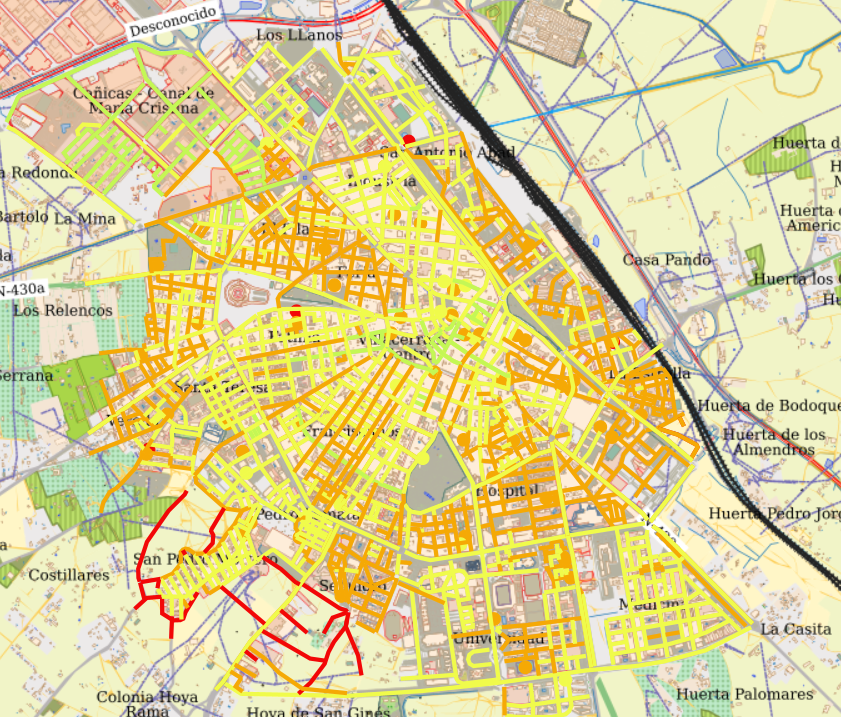
\includegraphics[width=\linewidth, height=55mm, keepaspectratio]{../capitulos/02-01-marco-legal/figuras/visor_albacete.png}
    \caption{Capa «Accesibilidad calles» del visor de Albacete.}
    \label{fig:mapa_albacete}
  \end{subfigure}\hfill
  \begin{subfigure}[t]{0.49\textwidth}\centering
    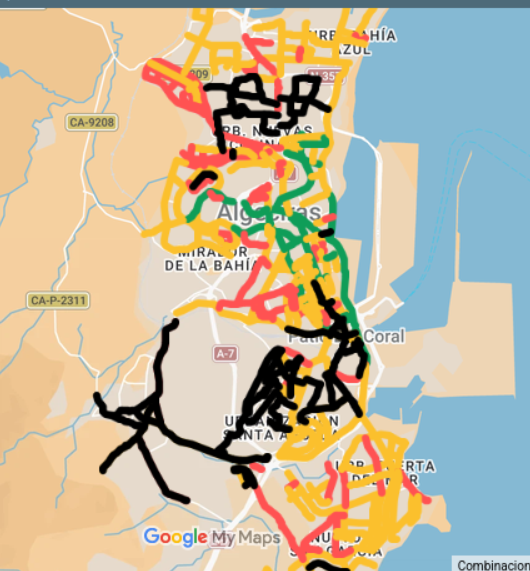
\includegraphics[width=\linewidth, height=55mm, keepaspectratio]{../capitulos/02-01-marco-legal/figuras/visor_algeciras.png}
    \caption{Visor de accesibilidad de Algeciras.}
    \label{fig:mapa_algeciras}
  \end{subfigure}
  \caption{Ejemplos de inventarios municipales de accesibilidad viaria.}
  \label{fig:inventarios_municipales}
  \fuente{(a) Ayuntamiento de Albacete (2026); (b) Ayuntamiento de Algeciras y ACCESIA (2026).}
\end{figure}

En los ejemplos de visualización, cada municipio ha diseñado su propia escala de categorías y colores para representar la accesibilidad de las vías urbanas, empleando colores rojos para indicar baja accesibilidad y colores verdes para indicar alta accesibilidad.

\subsection{Los planes de accesibilidad municipales}
¿Qué es un plan de accesibilidad universal (PAU), también conocido como plan de accesibilidad integral (PAI)?

Se trata de un documento técnico estratégico que se debe encargar por los ayuntamientos\footnote{RDL 1/2013, Disposición Adicional Cuarta.}, y que permite auditar, planificar, priorizar y presupuestar la eliminación de cualquier barrera un obstáculo que afecte a la accesibilidad universal, en las vías urbanas, transporte y espacios públicos del municipio.

Habitualmente tiene 4 fases diferentes:
\begin{enumerate}
    \item \textbf{Diagnóstico e inventario:} se debe realizar una inspección in situ para diagnosticar todos los elementos urbanos, como las vías, y analizar su accesibilidad. Se realizará un informe de campo detallado con las mediciones realizadas.
    \item \textbf{Propuestas:} se deben redactar las soluciones técnicas necesarias para eliminar las barreras detectadas en el diagnóstico, por cada elemento urbano.
    \item \textbf{Priorización:} determinar el orden de actuación de las medidas propuestas, priorizando aquellas con una mayor necesidad y un mayor impacto en la ciudadanía. En esta etapa se diferencian los plazos de ejecución (corto, medio y largo plazo).
    \item \textbf{Presupuesto:} realizar una valoración económica de las soluciones, generando un presupuesto global para el plan y un calendario de ejecución.
\end{enumerate}

Este desglose de fases es fundamental para el proyecto, puesto que permite conocer las necesidades de los municipios a la hora de elaborar los planes de accesibilidad, y demuestra que los datos de campo son la base para la toma de decisiones en las siguientes etapas del plan.
\\

Por otro lado, es importante considerar la posible diferenciación de las medidas y variables inspeccionadas en cada municipio, dado que los planes de accesibilidad no exigen seguir un formato único estandarizado y se adaptan a las particularidades de los consistorios.
\\

\subsection{Normativa de accesibilidad en edificios}
Aunque queda fuera del alcance del trabajo la clasificación de accesibilidad de los edificios, se indica a continuación cuáles son los puntos más importantes de la normativa, recogida en el Real Decreto 505/2007 (Ministerio de la Presidencia, 2007):
\begin{itemize}
    \item \textbf{Itinerarios accesibles:} se debe garantizar que las entradas principales de los edificios, así como sus aparcamientos, conecten sin barreras con los itinerarios peatonales accesibles.
    \item \textbf{Accesibilidad interior:} se exige que los espacios interiores del edificio, como pasillos o ascensores, sean accesibles para todas las personas, utilizando ascensores o rampas accesibles.
    \item \textbf{Utilización accesible:} se debe cumplir que todo el mobiliario fijo y los elementos informativos del edificio sea completo para todas las diversidades funcionales.
    \item \textbf{Seguridad:} se deben implementar medidas de seguridad que garanticen la protección de todas las personas, en caso de incendio, emergencia o evacuación.
\end{itemize}